% Code under BSD-3-Clause (see LICENSE). (c) 2026 Francesco Mario Antonio Mitrotta.
% Failure planes of a plane-stress unidirectional ply, adapted from Hashin (1980), Fig. 2.
% Axes: x1 along the fibres, x2 across them in the plane of the ply, x3 through the thickness
% (exaggerated). Arrows are the tractions for positive stresses.
% Build: pdflatex 01_hashin_failure_planes.tex
%        pdftocairo -png -r 200 -singlefile 01_hashin_failure_planes.pdf 01_hashin_failure_planes
\documentclass[tikz,border=4pt]{standalone}
\usetikzlibrary{arrows.meta}
\begin{document}
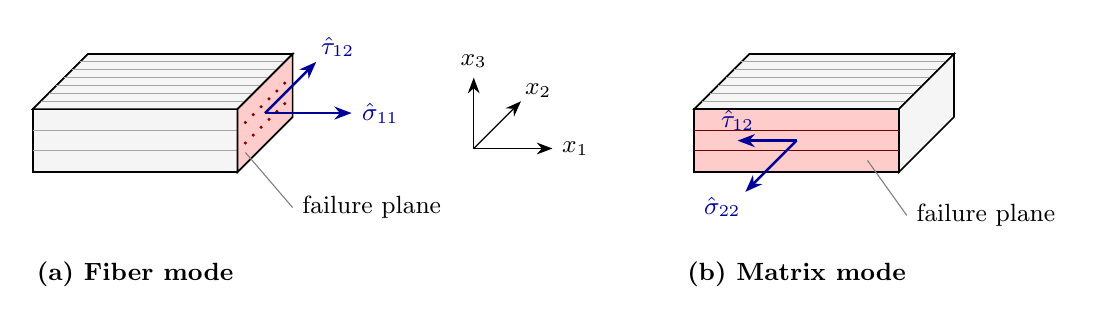
\begin{tikzpicture}[
    % oblique projection: tikz x = x1 (right, fibres), y = x2 (into the page), z = x3 (up, thickness)
    x={(1cm,0cm)}, y={(0.5cm,0.5cm)}, z={(0cm,1cm)},
    face/.style={draw=black, line width=0.6pt, fill=gray!8},
    plane/.style={draw=black, line width=0.6pt, fill=red!20},
    fibre/.style={gray!70, line width=0.4pt},
    load/.style={-{Stealth[length=2.2mm]}, line width=0.9pt, blue!60!black},
    lbl/.style={font=\small},
  ]
  \def\L{2.6}   % length along x1
  \def\W{1.4}   % width along x2
  \def\t{0.8}   % thickness along x3 (exaggerated)

  % ---------------- (a) fibre mode: the ply breaks across the fibres, plane normal to x1 ----------------
  \begin{scope}
    \filldraw[face] (0,0,0) -- (\L,0,0) -- (\L,0,\t) -- (0,0,\t) -- cycle;        % front face, x2 = 0
    \filldraw[face] (0,0,\t) -- (\L,0,\t) -- (\L,\W,\t) -- (0,\W,\t) -- cycle;    % top face, x3 = t
    \foreach \s in {0.2,0.4,...,1.21} \draw[fibre] (0,\s,\t) -- (\L,\s,\t);       % fibres on the top face
    \foreach \z in {0.27,0.53} \draw[fibre] (0,0,\z) -- (\L,0,\z);                % fibres on the front face
    \filldraw[plane] (\L,0,0) -- (\L,\W,0) -- (\L,\W,\t) -- (\L,0,\t) -- cycle;   % failure plane, x1 = L
    \foreach \s in {0.2,0.4,...,1.21} \foreach \z in {0.27,0.53}
      \fill[red!55!black] (\L,\s,\z) circle (0.6pt);                              % broken fibre ends
    \coordinate (C) at (\L,\W/2,\t/2);                                            % centre of the plane
    \draw[load] (C) -- ++(1.1,0,0) node[right, lbl] {$\hat\sigma_{11}$};
    \draw[load] (C) -- ++(0,1.3,0) node[above right=-2pt, lbl] {$\hat\tau_{12}$};
    \draw[gray] (\L,0.2,0.15) -- ++(0.6,0,-0.7) node[right, lbl, black] {failure plane};
    \node[lbl, font=\bfseries\small] at (\L/2,0,-1.3) {(a) Fiber mode};
  \end{scope}

  % ---------------- material axes ----------------
  \begin{scope}[xshift=5.6cm, yshift=0.3cm]
    \draw[-{Stealth[length=2mm]}] (0,0,0) -- (1.0,0,0) node[right, lbl] {$x_1$};
    \draw[-{Stealth[length=2mm]}] (0,0,0) -- (0,1.2,0) node[above right=-2pt, lbl] {$x_2$};
    \draw[-{Stealth[length=2mm]}] (0,0,0) -- (0,0,0.9) node[above, lbl] {$x_3$};
  \end{scope}

  % ---------------- (b) matrix mode: the ply splits along the fibres, plane normal to x2 ----------------
  \begin{scope}[xshift=8.4cm]
    \filldraw[face] (0,0,\t) -- (\L,0,\t) -- (\L,\W,\t) -- (0,\W,\t) -- cycle;    % top face, x3 = t
    \foreach \s in {0.2,0.4,...,1.21} \draw[fibre] (0,\s,\t) -- (\L,\s,\t);       % fibres on the top face
    \filldraw[face] (\L,0,0) -- (\L,\W,0) -- (\L,\W,\t) -- (\L,0,\t) -- cycle;    % end face, x1 = L
    \filldraw[plane] (0,0,0) -- (\L,0,0) -- (\L,0,\t) -- (0,0,\t) -- cycle;       % failure plane, x2 = 0
    \foreach \z in {0.27,0.53}
      \draw[fibre, red!45!black] (0,0,\z) -- (\L,0,\z);                           % fibres exposed along the crack
    \coordinate (M) at (\L/2,0,\t/2);                                             % centre of the plane
    \draw[load] (M) -- ++(0,-1.3,0) node[below left=-2pt, lbl] {$\hat\sigma_{22}$};
    \draw[load] (M) -- ++(-0.75,0,0) node[above, lbl] {$\hat\tau_{12}$};
    \draw[gray] (\L-0.4,0,0.15) -- ++(0.5,0,-0.7) node[right, lbl, black] {failure plane};
    \node[lbl, font=\bfseries\small] at (\L/2,0,-1.3) {(b) Matrix mode};
  \end{scope}
\end{tikzpicture}
\end{document}
